\chapter{Arhitektura i dizajn sustava}
		
		\textbf{\textit{dio 1. revizije}}\\

		Opis...

	
				
		\section{Baza podataka}
			
			\textbf{\textit{dio 1. revizije}}\\
			
		Za potrebe našeg sustava, odabrali smo relacijsku bazu podataka zbog njezine strukture koja olakšava modeliranje stvarnog svijeta. Osnovna građevna jedinica baze je relacija, odnosno tablica koja je identificirana imenom i skupom atributa. Glavna funkcija baze podataka je brza i jednostavna pohrana, izmjena i dohvat podataka za daljnju obradu. Baza podataka naše aplikacije uključuje sljedeće entitete:
		
		\begin{packed_item}
			\item  UserCustom		\textit{~ (korisnik)}
			\item  UserAuth			\textit{~ (prijava za korisnika)}
			\item  Advertisement	\textit{~ (oglas)}
			\item  Pet				\textit{~ (ljubimac)}
			\item  Picture			\textit{~ (slika)}
			\item  Message			\textit{~ (poruka)}
		\end{packed_item}
		
			\subsection{Opis tablica}
			
			
			\textbf{UserCustom}\hspace{10pt}Ovaj entitet sadržava sve važne informacije o korisniku aplikacije.
			Sadrži atribute: id (korisnički identifikacijski broj), username (korisničko ime), isShelter, firstName (ime korisnika), lastName (prezime korisnika), shelterName (ime skloništa ako je riječ o skloništu), email i phoneNumber (broj telefona). Ovaj entitet u vezi je 
			\textit{One-to-One} s entitetom UserAuth preko atributa username (korisničko ime korisnika),
			u vezi \textit{One-to-Many} s Message (poruka) preko korisničkog identifikacijskog broja,
			u vezi \textit{One-to-Many} s entitetom Advertisement preko korisničkog identifikacijskog broja (ili identifikacijskog broja skloništa).
			
				%Svjetlozelenom bojom označite primarni ključ. Svjetlo plavom označite strani ključ
				
				\begin{longtblr}[
					label=none,
					entry=none
					]{
						width = \textwidth,
						colspec={|X[6,l]|X[6, l]|X[20, l]|}, 
						rowhead = 1,
					} %definicija širine tablice, širine stupaca, poravnanje i broja redaka naslova tablice
					\hline \SetCell[c=3]{c}{\textbf{UserCustom}}	 \\ \hline[3pt]
					\SetCell{LightGreen}id & INT	&  jedinstveni brojčani identifikator korisnika	\\ \hline
					username & VARCHAR	&  jedinstveni identifikator korisnika	\\ \hline
					isShelter & BOOLEAN	&  oznaka je li korisnik sklonište	\\ \hline
					firstName & VARCHAR	&  ime korisnika	\\ \hline
					lastName & VARCHAR	&  prezime korisnika	\\ \hline
					shelterName & VARCHAR	&  ime skloništa	\\ \hline
					email & VARCHAR	&  e-mail adresa korisnika	\\ \hline
					phoneNumber & VARCHAR	&  broj telefona korisnika	\\ \hline
				\end{longtblr}
				
			\textbf{UserAuth}\hspace{10pt}Ovaj entitet sadržava sve što je potrebno kako bi se u sustav prijavio korisnik, a to je njegov username (korisničko ime) i password (pripadajuća loznika).Ovaj entitet je u vezi
			\textit{One-to-One} s entitetom UserCustom preko atributa username (korisničko ime).
			
				\begin{longtblr}[
					label=none,
					entry=none
					]{
						width = \textwidth,
						colspec={|X[6,l]|X[6, l]|X[20, l]|}, 
						rowhead = 1,
					} %definicija širine tablice, širine stupaca, poravnanje i broja redaka naslova tablice
					\hline \SetCell[c=3]{c}{\textbf{UserAuth}}	 \\ \hline[3pt]
					\SetCell{LightBlue}	username & VARCHAR &  jedinstveni identifikator korisnika  	\\ \hline
					password & VARCHAR	&  hash lozinke	\\ \hline
				\end{longtblr}
				
			
			\textbf{Advertisement}\hspace{10pt}Ovaj entitet sadržava sve važne informacije o oglasima koje će korisnici moći postavljati ili čitati.
			Sadrži atribute: id (identifikacijski broj oglasa), category (kategoriju), deleted (podatak o tome je li oglas izbrisan), dateTimeAdv (vrijeme oglašavanja), isInShelter (podatak o tome je li oglas ljubimca označen da je u skloništu), userId (ID korisnika), petId (ID ljubimca) i shelterId (ID skloništa).
			Ovaj entitet je u vezi
			\textit{Many-to-One} s entitetom UserCustom preko atributa userId i shelterId,
			u vezi \textit{One-to-Many} s entitetom Message preko identifikacijskog broja oglasa,
			u vezi \textit{One-to-Many} s entitetom Picture također preko identifikacijskog broja oglasa
			te u vezi \textit{Many-to-One} s entitetom Pet (ljubimcem) preko identifikacijskog broja ljubimca.
			
				\begin{longtblr}[
					label=none,
					entry=none
					]{
						width = \textwidth,
						colspec={|X[6,l]|X[6, l]|X[20, l]|}, 
						rowhead = 1,
					} %definicija širine tablice, širine stupaca, poravnanje i broja redaka naslova tablice
					\hline \SetCell[c=3]{c}{\textbf{Advertisement}}	 \\ \hline[3pt]
					\SetCell{LightGreen}	id & INT &  jedinstveni brojčani identifikator oglasa	\\ \hline
					category & ENUM	&  kategorije: lost, found, abandoned, sheltered, dead)	\\ \hline
					deleted & BOOLEAN	&  oznaka je li oglas izbrisan	\\ \hline
					dateTimeAdv & TIMESTAMP	&  vrijeme postavljanja oglasa	\\ \hline
					isInShelter & BOOLEAN	&  oznaka je li ljubimac smješten u sklonište	\\ \hline
					\SetCell{LightBlue} userId & INT	&  jedinstveni brojčani identifikator korisnika	\\ \hline
					\SetCell{LightBlue} petId & INT	&  jedinstveni brojčani identifikator ljubimca	\\ \hline
					\SetCell{LightBlue} shelterId & INT	&  jedinstveni brojčani identifikator skloništa	\\ \hline
				\end{longtblr}
				
				
			
				
				
			
			\subsection{Dijagram baze podataka}
				
				%unos slike
				\begin{figure}[H]
					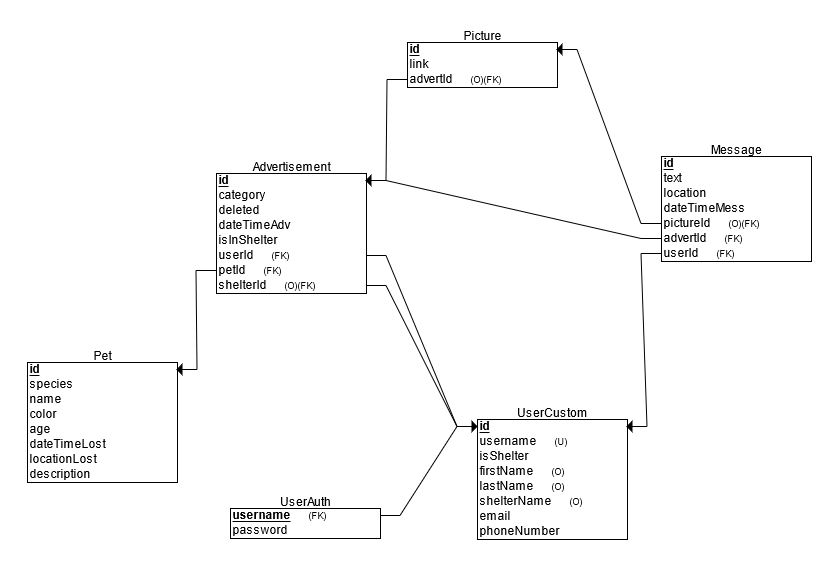
\includegraphics[scale=0.63]{dijagrami/dijagramBaze/relacijskiModel.PNG} %veličina slike u odnosu na originalnu datoteku i pozicija slike
					\centering
					\caption{Relacijski dijagram baze podataka}
					\label{fig:relDijagram}
				\end{figure}

				\begin{figure}[H]
					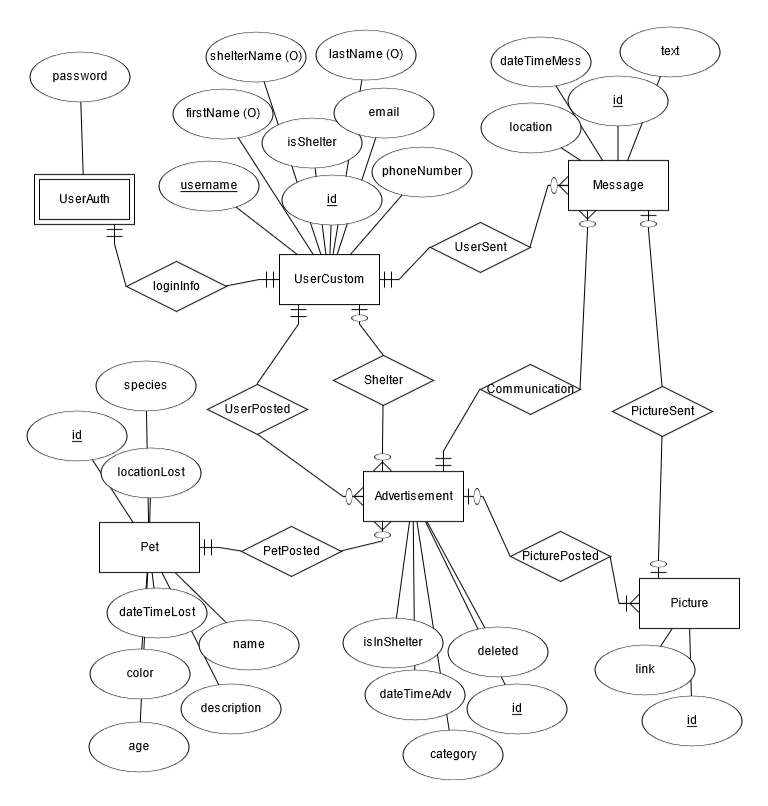
\includegraphics[scale=0.65]{dijagrami/dijagramBaze/ERmodel.PNG} %veličina slike u odnosu na originalnu datoteku i pozicija slike
					\centering
					\caption{E-R dijagram baze podataka}
					\label{fig:erDijagram}
				\end{figure}

			\eject
			
			
		\section{Dijagram razreda}
		
			\textbf{\textit{dio 1. revizije}}\\
			
			Otprilike...
			
			\textbf{\textit{dio 2. revizije}}\\			
			
			Točno...
			
			\eject
		
		\section{Dijagram stanja}
			
			
			\textbf{\textit{dio 2. revizije}}\\
			
			Ne sad...
			
			
			\eject 
		
		\section{Dijagram aktivnosti}
			
			\textbf{\textit{dio 2. revizije}}\\
			
			Ne sad...
			
			\eject
		\section{Dijagram komponenti}
		
			\textbf{\textit{dio 2. revizije}}\\
		
			Ne sad...